\section {Software Architecture}

The simulation is built on top of ROSS. 
As shown in figure \ref{fig:software}, the application consists of four major modules, Aircraft, Weather/Disaster, Airport and Region Controller. 
Aircrafts are sent between the airport and the region controller. Airport and region controller access to the Weather/Disaster module upon a request. 
Airport contains a local traffic manager, which checks the number of runways in use. 
The local traffic manager computes a taxi in/out time and calculate a delay based on the airport size.
Region controller contains an air traffic manager, which tracks the number of airplanes in the region.
The controller handles a hand-off request and computes a hand-off time/delay based on the weather condition and the current capacity of airplanes in the region. 
The controller follows the hand-off protocol to transit an airplane from one region to the next region.  
Due to the limitation of using arrays in Backstroke, we used Backstroke random number generator which performs a state-saving for a random seed using a stack instead of ROSS random number generator.


\begin{figure} [htd]
\centering
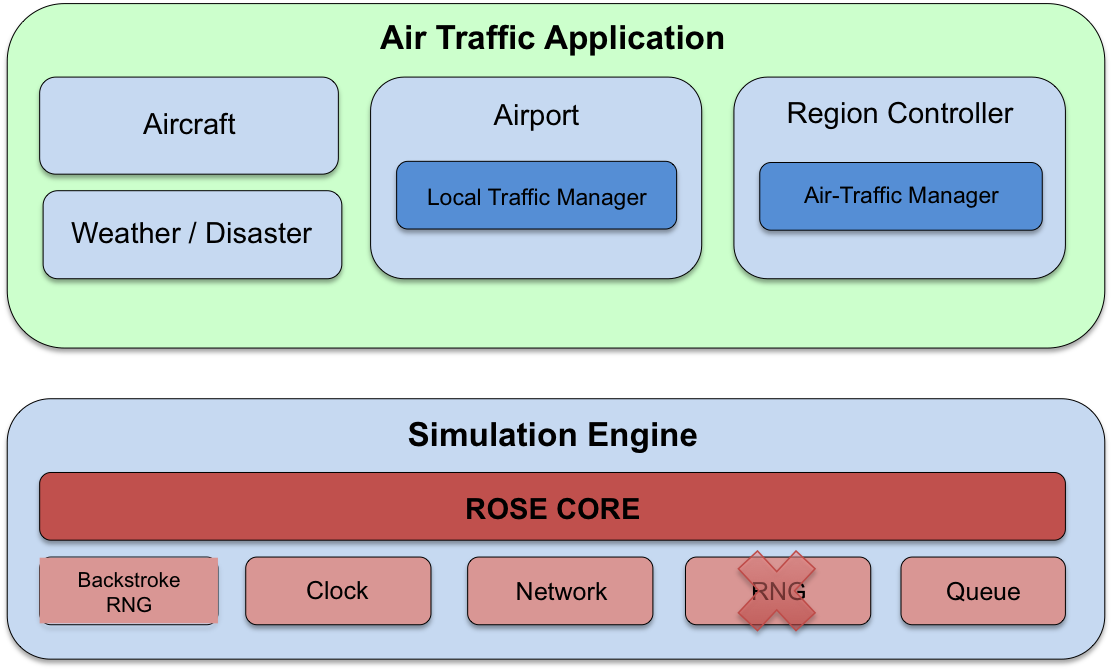
\includegraphics[width=4.2in]{/Users/chayong/Documents/project2/figs/software.png}
\caption{Software Architecture of Air Traffic Simulation}
\label{fig:software}
\end{figure}
